\documentclass[15pt]{report}
\usepackage{amsmath}
\usepackage{amsfonts}
\usepackage{amssymb}
\usepackage{graphicx}
\usepackage{wrapfig}
\usepackage{enumitem}
\usepackage{listings}
\title{Evaluating Newton's Method to find Real and Complex roots of Various Functions}
\author{By Rounak Jangir \\Prashant Verma\\ Aditya Prakash \\Akhilesh Kumar\\ Manu Sharma \\Shubham Sharma }
\begin{document}
\maketitle
\newpage
{\huge$\star$ Abstract $\star$}\\
\noindent\rule{12 cm}{1 pt}\\ \\ \\
In our exploratory project, we evaluated Newton’s method (Newton Raphson Method) for finding out real and complex roots of polynomial functions, and analysed the resulting Newton basins of Attraction. A Newton basin is the set of points (initial guesses) for which Newton’s method converges to a particular solution. We took different examples of polynomial functions, calculated their roots (both real and complex) using Newton's method and evaluated the resulting Newton basins.
We also explored the different applications of Newton's method.
\newpage

{\huge$\star$ Introduction $\star$}\\
\noindent\rule{12 cm}{1 pt}\\ \\
Our Project involves the exploration and use of Newton Raphson’s method (Newton’s Method) and its properties. We used Newton's method to evaluate the real and complex  roots of polynomial functions and then analysed the resulting Newton basins of Attraction. We experimented with various polynomial functions. We also studied and explored the various applications of Newton's method. Using the high level language OCTAVE which is used for mathematical computation, we were able to compute the Newton basins and were able to appreciate the Newton's method and the role and power of computation in Mathematics.
\newpage 

{\huge$\star$ Newton's Method $\star$}\\
\noindent\rule{12cm}{1 pt}\\ \\
In order to obtain the roots of various polynomials, we can use Newton's Method.
We use Newton's method to approximate the solution (both real and complex) of f(x)=0 where \textit{f} is a polynomial function.\\
Newton’s method is a numerical and iterative algorithm for finding the zeros (or roots) of a function (of the form f(x)=0). It is a easy method to understand and is very efficient and powerful technique in approximation of roots.\\ \\
Let f(x) be a good function and \textit{p} be a root of a function.We start with an estimate $x_{0}$ which is close to \textit{p}. Now, by using $x_{0}$, we produce an improved approximation (or we think we improved) $x_{1}$. From $x_{1}$, we produce another estimate $ x_{2}$ . We go on further and further, until we get really close to \textit{p} or it becomes clear that we are getting nowhere.\\
The Newton-Rhapson method works really good if the initial 'guess' is very close to root for a well defined function. But, it can go drastically wrong in other cases.\\

Now, let $x_{0}$ be very close to the root \textit{p}. Then, suppose p=$x_{0}$+h. Here, \textit{h} shows how far the guess is from the root.
Since, h is infinitesimally small, so we can apply linear approximation here,\\ \\
0=f(p)=f($x_{0}$+h)$\approx$f($x_{0}$)+ hf'($x_{0}$)\\ \\
If f'($x_{0}$)$\approx$=0\\ \\
h $\approx$ -$\dfrac{f(x_{0})}{f'(x_{0})}$\\ \\
Therefore, p= $x_{0}$+h $\approx$ $x_{0}$ -$\dfrac{f(x_{0})}{f'(x_{0})}$\\ \\
Our better approximation becomes \\ $x_{1}$=  $x_{0}$ -$\dfrac{f(x_{0})}{f'(x_{0})}$\\ \\
On generalising,we have \\ \\ $x_{n+1}$=  $x_{n}$ -$\dfrac{f(x_{n})}{f'(x_{n})}$\\ \\ \\
\section*{Geometric Interpretation}
In Newton's Method, we start with an initial guess that is close to a root. We then approximate the function using it's tangent line and then the x-intercept is computed. This x-intercept will be a better approximation of the root of the equation rather than the original guess. The method is repeated again with the x-intercept. This method is repeated again and again until the ultimate solution is obtained (or a solution which is very close to the real root). More iterations will result in a more closer solution to the real/complex root.  \\ \\
\begin{figure}[h]
\centering
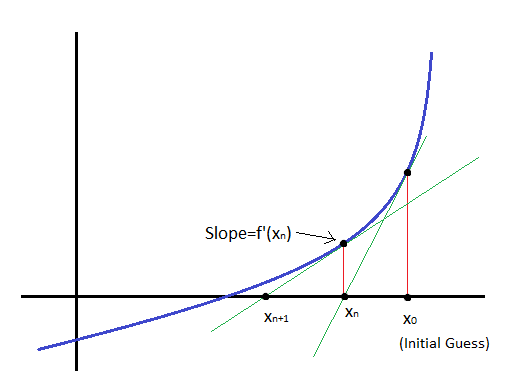
\includegraphics[width=1 \columnwidth]{1}
\caption{Iteration of Newton's Method}
\end{figure}\\ \\
Suppose f : [a, b] $\rightarrow$ R is a differentiable function defined on [a, b] $\rightarrow$ R. Formula for the Newton's methods can be derived very easily. Suppose we have a initial guess $x_{n}$. Then we can derive a better approximation. The equation of the tangent to the curve y = f(x) at the point $x=x_{n}$ is\\ \\
{\textbf{\Large $y=f'(x_{n})(x-x_{n})+f(x_{n})$}}\\ \\
where f'(x) denotes the derivative of the function \textit{f}.
The x-intercept of this line (distance of the point from the origin where this line cuts the x-axis i.e. y=0) is then used as the next approximation of the root, $x_{n+1}$. Replacing x by $x_{n+1}$ and setting y=0, we get,\\ \\
{\textbf{\Large $0=f'(x_{n})(x_{n+1}-x_{n})+f(x_{n})$}}\\ \\
solving for $x_{n+1}$ we get,\\ \\
{\textbf{\Large $x_{n+1}$=$x_{n}-\dfrac{f(x_{n})}{f'(x_{n})}$}}\\ \\

We start the process with some arbitrary value $x_{0}$. The closer to the root of the equation we are, the better. But in case of no initial idea, any value can be taken. This method usually converges for the guesses closer to the roots. But some exceptions are there where Newton's method doesn't converge. They will be discussed later.
The set comprising of all the initial guesses for which there is a particular solution having the Newton's method converging on it is called a Newton Basin.
The set comprising of all the initial guesses for which, within a specified number of iterations the Newton's method does not converge is called the Newton Wasteland.

The geometric interpretation of complex case is analogous to the real case. 
{\textbf{\Large $x_{n+1}$=$x_{n}-\dfrac{f(x_{n})}{f'(x_{n})}$}}\\ \\
This equation can be substituted for the complex function as\\
{\textbf{\Large $z_{n+1}$=$z_{n}-\dfrac{f(z_{n})}{f'(z_{n})}$}}\\ \\
The roots of a curve can be found by the following method
\begin{itemize}
\item First the initial guess $Z_{k}$ is taken and the value of the function is found of the curve.
\item Then,the equation of the tangent plane $T_{1}$ is computed on that point found on the curve.
\item The intersection of the plane $T_{1}$ and the x-y plane gives the equation of a line L.
\item A perpendicular is drawn from the initial guess $Z_{k}$ point to the line L obtained in the previous step.
\item The foot of perpendicular thus obtained gives the better approximation of the root of the complex function.

\end{itemize}
The gradient of the function at $Z_{k}$ is given by the opposite direction of the $Z_{k+1}$-$Z_{k}$.\\ \\

\newpage
{\textbf{\underline{\Large Examples}}}\\ \\
{\large \textbf{1.\hspace*{5mm}\textit{f(x)=$x^{2}-16$=0}}}\\ \\ 
Suppose we want to solve for the given function f(x)=$x^{2}-16=0$. The graph of the function is given below:\\ 
\begin{figure}[h]
\centering
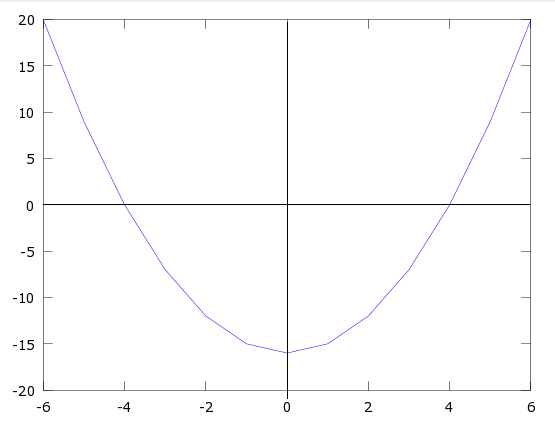
\includegraphics[width = 0.8 \columnwidth]{3}
\caption{Polynomial $x_{2}-16=0$}
\label{fig:Eg. 1}
\end{figure}\\ \\
From the above figure, we can easily make out that the roots of function \textit{f} are 4 and -4. Since\\
{\large f(x)=$x^{2}-16=0$\\
\hspace*{6mm}=(x-4)(x+4)=0\\
\hspace*{6mm}=$\pm$4}\\ \\
Now, using Newton’s method to solve, we iteratively use formula derived for the Newton's Method to approximate x such that f(x)=0. Let us take $x^{0}=5$. We then apply Newton's method to obtain the closer approximation.\\ \\
{\large $x_{1}=x_{0}-\dfrac{f(x_{0})}{f'(x_{0})}$ \hspace*{20 mm} f(x)=$x^{2}-16$ \hspace*{20mm}  f'(x)=2x}\\ \\
$\Rightarrow$ {\large $x_{1}=5-\dfrac{f(5)}{f'(5)}$} \\ \\
$\Rightarrow$ {\large $x_{1}=5-\dfrac{9}{10}$}\hspace*{20mm}$\Rightarrow$ {\large $x_{1}=4.1$}\\ \\
Similarly now for $x_{2}$ \\ \\
{\large $x_{2}=x_{1}-\dfrac{f(x_{1})}{f'(x_{1})}$}\\ \\
$\Rightarrow$ {\large $x_{2}=4.1-\dfrac{f(4.1)}{f'(4.1)}$} \\ \\
$\Rightarrow$ {\large $x_{2}=4.1-\dfrac{0.81}{8.2}$} \hspace*{20mm} $\Rightarrow$ {\large $x_{1}=4.001$}\\ \\
which is a much better approximation than $x_{1}$. Similarly, by repeating Newton's Method iteratively, we will eventually find the root of the function or a much better approximation.\\ \\ \\ \\
{\large \textbf{2.\hspace*{5mm}\textit{f(x)=$x^{2}-4x+4$=0}}}\\ \\
Suppose we want to solve for the given function f(x)=$x^{2}-4x+4$=0. The graph of the function is given below:\\
\begin{figure}[h]
\centering
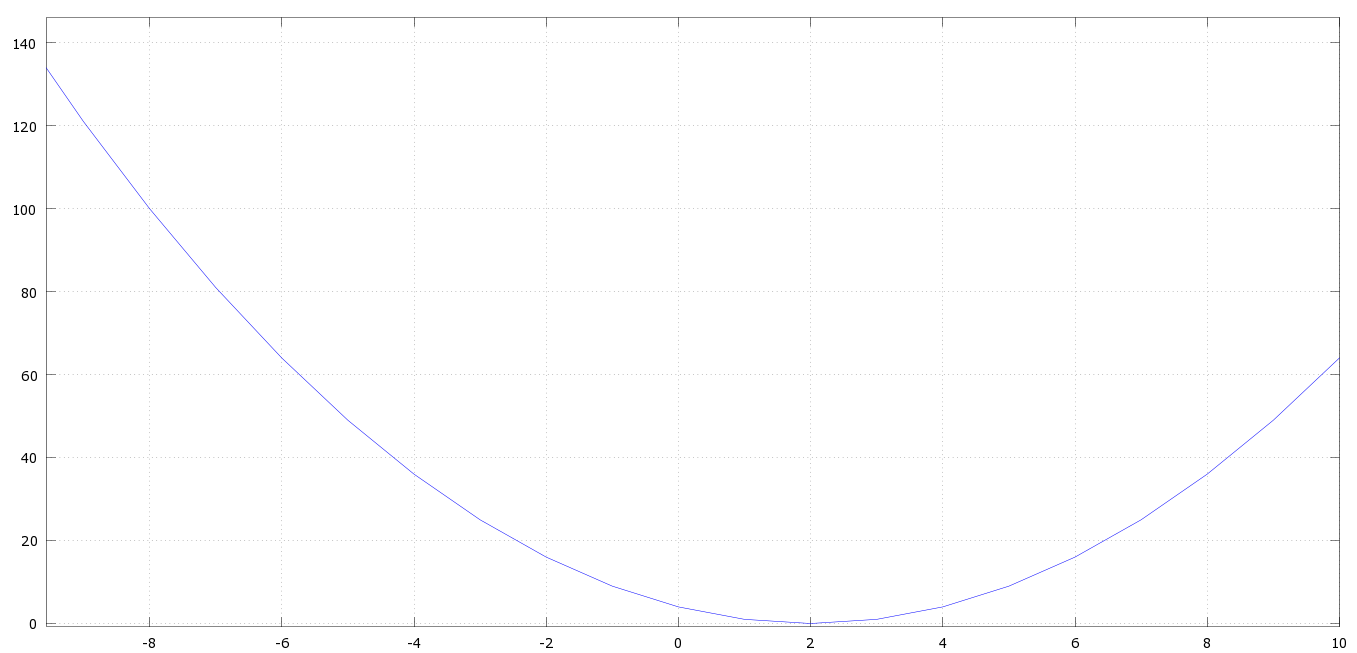
\includegraphics[width = 1.2 \columnwidth]{4}
\caption{Polynomial $x^{2}-4x+4$=0}
\label{fig:Eg. 2}
\end{figure}\\ \\
From the above figure, we can easily make out that the root of function \textit{f} is 2. Root 2 have a multiplicity of 2. Since\\
{\large f(x)=$x^{2}-4x+4$=0\\
\hspace*{6mm}=$x^{2}-2x-2x+4=0$\\
\hspace*{6mm}=x(x-2)-2(x-2)=0\\
\hspace*{6mm}=(x-2)(x-2)\\
\hspace*{6mm}=2}\\ \\
Now, using Newton’s method to solve, we iteratively use formula derived for the Newton's Method to approximate x such that f(x)=0. Let us take $x^{0}=3$. We then apply Newton's method to obtain the closer approximation.\\ \\
{\large $x_{1}=x_{0}-\dfrac{f(x_{0})}{f'(x_{0})}$ \hspace*{20 mm} f(x)=$x^{2}-4x+4$ \hspace*{20mm}  f'(x)=2x-4}\\ \\
$\Rightarrow$ {\large $x_{1}=3-\dfrac{f(3)}{f'(3)}$} \\ \\
$\Rightarrow$ {\large $x_{1}=3-\dfrac{1}{2}$}\hspace*{20mm}$\Rightarrow$ {\large $x_{1}=2.5$}\\ \\
Similarly now for $x_{2}$ \\ \\
{\large $x_{2}=x_{1}-\dfrac{f(x_{1})}{f'(x_{1})}$}\\ \\
$\Rightarrow$ {\large $x_{2}=2.5-\dfrac{f(2.5)}{f'(2.5)}$} \\ \\
$\Rightarrow$ {\large $x_{2}=2.5-\dfrac{0.25}{1}$} \hspace*{20mm} $\Rightarrow$ {\large $x_{1}=2.25$}\\ \\
which is a much better approximation than $x_{1}$. Similarly, by repeating Newton's Method iteratively, we will eventually find the root of the function or a much better approximation.\\ \\ \\ \\
\newpage
\section*{Limitations of Newton's method}
\subsection*{Bad Starting Point}
This kind of limitation happens when the choice of starting point is wrong. Sometimes, a good function satisfies all the conditions necessary for convergence but the starting point is chosen wrong. This happens because most probably that point point doesn't lie in the interval where the function converges.   
\begin{enumerate}
\item \textbf{Iterative point is stationary}\\If a stationary point of a function is encountered (i.e. the value of f'(x)=0), then the method will give the next iteration as infinity. It means, the method will give a wrong result. For eg. \\ \\
Consider the function:\\
\hspace*{15mm} f(x)$=$ 4$-x^{2}$ \\
The solutions of the function f(x)$=$0 are at x $=$ $\pm$2. Let us take x$_{0}$ $=$ 0 as our starting point. 
for f(x)$=$ 4$-x^{2}$, f'(x) $=$ 2x\\
Therefore, \\
x$_{1}$ $=$ x$_{0}$ $-$ $\dfrac{f(x_{0})}{f'(x_{0})}$ \\ \\
Now for x$_{0}$ $=$ 0, f'(x$_{0}$) $=$ 0,   \\
x$_{1}$ $=$ x$_{0}$ $-$ $\dfrac{f(x_{0})}{f'(x_{0})}$ $=$ 0 $-$ $ \dfrac{4}{0} $ $\approx$ $\infty $ \\ \\
The same issue will occur if instead of this point, any other iterative point is chosen which is stationary. Hence, in this example, 0 is the stationary point for this function f(x). \\

\item \textbf{Starting point enters a cycle}\\ In some cases, the starting points sometimes enter a infinite cycle, where \\
\hspace*{20mm}$x_{k}$=$x_{k+p}$  \hspace*{20mm} where p is natural number.\\
i.e. The values of newton's iterations repeats themselves after a certain interval of iterations. For eg. \\ \\
Consider a function: \\
f(x)$=$ x$^{3}$ $-$ 2x $+$ 2\\
Therefore, f'(x)$=$ 3x $-$ 2\\ \\
Let x$_{0}$ $=$ 0. Therefore, \\ \\
x$_{1}$ $=$ x$_{0}$ $-$ $\dfrac{f(x_{0})}{f'(x_{0})}$ $=$ x$_{1}$ $=$ 0 $-$ $\dfrac{f(0)}{f'(0)}$ \\
x$_{1}$ $=$ 0 $-$ $\dfrac{2}{-2}$ $=$ x$_{1}$ $=$ 1\\ \\
Similarly,\\ \\
x$_{2}$ $=$ 1 $-$ $\dfrac{f(1)}{f'(1)}$ $=$ x$_{2}$ $=$ 1 $-$ $\dfrac{1}{1}$ $=$ x$_{2}$ $=$ 0\\ \\

Consider a function f(x)=$e^{x}$ $-$ 2x=0.\\ \\
Therefore,f'(x) $=$ $e^{x}$ $-$ 2.\\ \\ 
Let $x_{0}$ $=$ 1,we get\\ \\ 
$x_{n+1}$ $=$ $x_{n}$ - $\dfrac{e^{x_{n}} - 2x_{n}}{e^{x_{n}} - 2}$\\ \\
$x_{1}$ $=$ 1 $-$ $\dfrac{f(1)}{f'(1)}$ $=$ 1 $-$ 1 $=$ 0 \\ \\


We observe that the first iteration produces 1 and second iteration produces 0. This concludes that the sequence now alternates between these two values without actually converging to the root. 
\end{enumerate}
\subsection*{Derivative Issues}
The function has to be continuously differentiable in the neighbourhood of the root for the Newton's Method to work. If it is not, Newton's method will always diverge or fail except in the lucky case in which solution is obtained on the first guess.
\begin{enumerate}
\item If the function f(x) is not differentiable in the neighbourhood of root, then the newton method will give false results.\\
\item If the derivative of the function does not exist at the roots, then the next iterations will not converge to the roots, instead the distance between the root and $x_{k+1}$ increases. For eg. \\ \\
Consider the function:\\ 
f(x)$=$ x$^{\dfrac{1}{3}}$\\ \\
Therefore,\\
x$_{n+1}$ $=$ x$_{n}$ $-$ $\dfrac{x_n^{\dfrac{1}{3}}}{\dfrac{1}{3}x_n^{\dfrac{1}{3}-1}}$ $=$ x$_{n}$ $-$ 3x$_{n}$ $=$ -2x$_{n}$\\
Thus, we observe that the after each iteration, distance gets doubled from the solution. As also visible, it overshoots the value  and lands on the side opposite to the side of the y$-$axis where the iterative point is. In fact, it is clearly visible that the iterations diverges towards infinity.
\end{enumerate}

\section*{Applications of Newton's Method}
\subsection*{Minimization and maximization problems}
Newton's Method can be used to find the maxima or minima  for a function. The derivative is zero at the minimum or maximum, therefore Newton's Method can be applied to the derivative of the function to find maxima or minima. Note that Newton's method only gives the value. Further calculations have to be made to find whether it is a maxima or minima. The iteration becomes:\\ \\
x$_{n+1}$ $=$ x$_{n}$ $-$ $\dfrac{f'(x_{n})}{f''(x_{n})}$\\
\subsection*{Multiplicative inverse of numbers}
Newton's Method can be used to find the reciprocal of a number using only subtraction and multiplication. It is an important application of this method.\\
Consider the number D whose reciprocal is to be found out. Let \textit{x} be it's reciprocal. Therefore, \\
D$=$ $\dfrac{1}{x}$ $=$ Dx $=$ 1\\
Therefore, to find the reciprocal of the number D amounts to finding the solution of the equation:\\
f(x)=Dx-1 $\Longrightarrow$ f(x) $=$ D $-$ $\dfrac{1}{x}$\\ \\
Newton's iteration will be:
x$_{n+1}$ $=$ x$_{n}$ $-$ $\dfrac{f(x_{n})}{f'(x_{n})}$\\
x$_{n+1}$ $=$ x$_{n}$ $-$ $\dfrac{D-\dfrac{1}{x_{n}}}{\dfrac{1}{x_{n}^{2}}}$ \\
x$_{n+1}$ $=$ x$_{n}$(2$-$Dx$_{n}$)\\ \\	
\section*{Rate}
For general iterative methods, define error at iteration \textit{n} by \\
$e_{n}$ = $x_{n}$– R, where $x_{n}$ is approximate solution and R is true solution.\\For methods that maintain interval known to contain solution, rather than specific approximate value for solution, take error to be length of interval containing solution.

Sequence converges with rate \textit{r} if\\
$lim_{n\rightarrow \infty}$ $\dfrac{e_{n+1}}{{\vert e_{n} \vert}^r}$ $=$ C \\for some finite non zero constant C. \\
If r=1, the rate of divergence is linear. Similarly if r=2, the rate of convergence is quadratic.\\ \\
If R $=$ g(R) and $\vert g'(R) \vert$ $<$ 1, then there is an interval containing R such that iteration \\
\hspace*{40mm} x$_{n+1}$ $=$ g(x$_{n}$)\\
converges to R if started within that interval.\\ \\
Representing Newton's Method as above,\\
\hspace*{30mm}x$_{n+1}$ $=$ x$_{n}$ $-$ $\dfrac{f(x_{n})}{f'(x_{n})}$ $=$ g(x$_{n}$)\\
Therefore for Newton's Method, Condition for convergence is\\  
\hspace*{40mm} $\vert g'(x) \vert$= $\vert\dfrac{f(x)f"(x)}{{[f'(x)]}^2  }\vert <$  1\\
If $\vert g'(x) \vert > $1, then  the newton's method do not converges to any root.\\
\subsubsection*{Convergence rate of Newton's method}
R $-$ x$_{n+1}$ $=$ g(R) $-$ g(x$_{n}$)\\
because R $=$ g(R) and x$_{n+1}$ $=$ g(x$_{n}$)\\ \\
Using Taylor Expansion, we can write,\\
g(x$_{n}$) $=$ g(R) $+$ g'(R)$\dfrac{(R-x_{n})}{1!}$ $+$ g''(R)$\dfrac{(R-x_{n})^{2}}{2!}$ $+$ g''(R)$\dfrac{(R-x_{n})^{3}}{3!}$ $+$ ... \\
Ignoring higher order terms, we get\\
g(x$_{n}$) $=$ g(R) $+$ g'(R)(R$-$x$_{n}$) $+$ g''(R)$\dfrac{(R-x_{n})^{2}}{2}$\\ \\
$\vert g'(x) \vert$= $\vert\dfrac{f(x)f"(x)}{{[f'(x)]}^2  }\vert$\\ \\
Now for R,\\ 
$\vert g'(R) \vert$= $\vert\dfrac{f(R)f"(R)}{{[f'(R)]}^2  }\vert$\\ \\
and f(R)$=$0 because R is the true solution of function \textit{f}.\\
Therefore,\\ 
$\vert g'(R) \vert$=0 \\ \\
g(x$_{n}$) $=$ g(R) $+$ g''(R)$\dfrac{(R-x_{n})^{2}}{2}$\\ \\
x$_{n+1}$ $=$ R $+$ g''(R)$\dfrac{(R-x_{n})^{2}}{2}$\\ \\
x$_{n+1}$ $-$ R $=$ g''(R)$\dfrac{(R-x_{n})^{2}}{2}$\\ \\
e$_{n+1}$ $=$ g''(R)$\dfrac{e_{n}^{2}}{2}$\\ \\
$\dfrac{\vert e_{n+1} \vert}{\vert e_{n}\vert^{2}}$ $=$ $\dfrac{g''(R)}{2}$\\ \\
$\dfrac{g''(R)}{2}$ $=$ C, where C is a finite non zero constant.
Therefore,\\ \\
$\dfrac{\vert e_{n+1} \vert}{\vert e_{n}\vert^{2}}$ $=$ C\\
and we know that,\\ \\
$lim_{n\rightarrow \infty}$ $\dfrac{\vert e_{n+1}\vert}{{\vert e_{n} \vert}^r}$ $=$ C \\ \\
which implies \textit{r} $=$ 2. Therefore, Newton's Method is \textbf{quadratically convergent}. 
\newpage
\section*{Using Octave as Mathematical Computational tool}
In order the illustrate the Newton's Basins of Attraction for a given polynomial, we need a software which can implement these calculations and plot basins accordingly. The software we have used is Octave.\\
\subsection*{What is Octave?}
Octave, mostly known as GNU Octave is a high-level programming language, which is primarily intended for numerical computations. It provides a command line interface to solve linear and non-linear problems numerically. This language is mostly compatible with MATLAB, which is another high-level programming language which serves the same purpose but is more vast and can be used for more purposes also. GNU Octave takes fraction of time to solve and compute numerical computations than in other languages like C, C++, Java etc. Octave language is an interpreted programming language and supports many common C standard library functions. Octave is made available under the GNU General Public License, therefore it is freely available. Octave has a built-in compatibility for complex numbers  and have powerful built-in math functions. Therefore, Octave seemed to be the best suitable language for illustrating Newton Basins of Attraction.
\newpage
\section*{Octave Computational Results}
We used Octave to find the roots(real or complex) of the polynomial, show the sequential iteration of a number towards any of the root of the polynomial and finally, to illustrate Newton Basins of Attraction for some polynomials of different degrees.\\
\subsubsection*{Newton Basins of Attraction}
As discussed earlier, Newton Basin is a set of initial guesses for which Newton's method converges to a particular root of the polynomial. Below illustrated are Newton Basins for different polynomials of different degrees.   
\newpage
\section*{Conclusion}
Using power of computation and Octave, we computed and analysed Newton Basins and wastelands for different polynomials. We further analysed the sequential iteration of Newton's method for an initial guess towards a root of the polynomial using Octave.
\newpage
\section*{References}
\begin{itemize}
\item Wikipedia, `Newton's Method' \\$http://en.wikipedia.org/wiki/Newton's\_method$
\item David E. Joyce, `Newton's Method and Basins'\\$http://aleph0.clarku.edu/\sim djoyce/newton/method.html$
\item Jonathan S. Renning, `Convergence rate of Newton's Method'\\$http://www.math-cs.gordon.edu/courses/ma342/handouts/rate.pdf$
\item Courtney Watts, `Evaluating Newton's method for real and complex roots of various polynomials\\
$http://cms.uhd.edu/faculty/redlt/cwseniorproject.pdf$
\end{itemize}

   
\end{document}

